% Executive report: Applied Data Science Project with Python (UAB, 2026-2027)
% Build with `just report` (needs latexmk + a TeX distribution) or upload to Overleaf.
\documentclass[11pt,a4paper]{article}

\usepackage[utf8]{inputenc}
\usepackage[T1]{fontenc}
\usepackage[margin=2.5cm]{geometry}
\usepackage{graphicx}
\usepackage{booktabs}
\usepackage{amsmath,amssymb}
\usepackage{hyperref}
\usepackage{xcolor}

% Figures produced by the pipeline are saved in figures/
\graphicspath{{figures/}}

\title{US Air Quality: Multi-Station Aggregation \& Pollution Forecasting}
\author{TODO: Member 1 \and Member 2 \and Member 3 \and Member 4}
\date{Master in Modelling for Science and Engineering --- \today}

\begin{document}
\maketitle

\begin{abstract}
TODO: 150--200 words. Problem, data, approach, headline result.
\end{abstract}

\section{Introduction \& Problem Statement}
% Context of the US Pollution dataset (EPA, 2000--2016, NO2/O3/SO2/CO).
% Task type: supervised regression / spatiotemporal forecasting of next-day AQI.
% Analytical hypotheses and team goals.

\section{Data Cleaning \& Feature Engineering}

The raw file has 1{,}746{,}661 rows and 29 columns, covering 204 stations from
January 2000 to May 2016. The first exploration is in
\texttt{notebooks/01\_data\_exploration.ipynb}; the cleaning is implemented in
\texttt{src/applied\_data\_science\_ri/cleaning.py}.

\paragraph{Loading and memory.} Read with default types, the file takes 607\,MB in
memory. Storing repeated text (state, county, city, units) as \texttt{category},
measurements as \texttt{float32}, and skipping the redundant row-index column
reduces it to 178\,MB.

\paragraph{Duplicated rows.} A station-day appears on 4 rows on average (up to 324).
NO\textsubscript{2} and O\textsubscript{3} are identical across the copies; only
SO\textsubscript{2} and CO change, because they are measured with several methods
and the file contains every combination of them. We collapse each station-day into
a single row: means and AQIs are averaged over the methods and the daily maximum
keeps the highest value. This leaves about 413{,}000 station-days.

\paragraph{Missing values.} Before deduplication, SO\textsubscript{2} and CO AQI were
missing in exactly 50\% of rows: only one of the methods reports the AQI. Since the
average skips missing values, this gap disappears after deduplication. Each station
is then given one row per calendar day between its first and last measurement, so
that ``$k$ days before'' always means $k$ calendar days. Days on which a station did
not report (18.4\%) are left as missing rather than filled in, to avoid inventing
data. How to handle them is left to the modelling stage.

\paragraph{Units and invalid values.} Each pollutant uses a single unit, so no
conversion is needed. Small negative concentrations (down to $-2$\,ppb; 22{,}690 rows
for SO\textsubscript{2}) are physically impossible and most likely sensor noise
around zero, so they are set to 0. Rows from ``Country Of Mexico'' are removed, as
the study is about the US.

\paragraph{Features.} The task is to forecast the O\textsubscript{3} AQI of the next
day at each station using only information available today
(\texttt{features.py}). Based on the EDA we build:
\begin{itemize}
  \item \textbf{Past values:} the AQI of each pollutant 1, 2, 3, 7, 14 and 28 days
        before, and the mean O\textsubscript{3} AQI over the last 3, 7 and 30 days.
  \item \textbf{Calendar:} month, day of the week, weekend flag, and the day of the
        year encoded as $\sin$/$\cos$ so that December and January are close.
  \item \textbf{Spatial:} the mean O\textsubscript{3} AQI of the \emph{other}
        stations of the same state on the same day (the station itself is excluded).
\end{itemize}
All shifts and rolling windows are computed per station, so values from different
stations never mix. The final table has 410{,}271 rows and 49 features.

\section{Exploratory Data Analysis \& Visual Storytelling}
% Figures are generated by `just run eda` from the cleaned data.

\paragraph{Station coverage.} The number of stations reporting changes strongly
through the year (Figure~\ref{fig:coverage}): around 80 stations report in summer
but only about 45 in winter, probably because ozone is often only monitored during
the warm season. The data therefore has systematic winter gaps. The drop at the end
is only the end of the dataset (May 2016).

\begin{figure}[h]
  \centering
  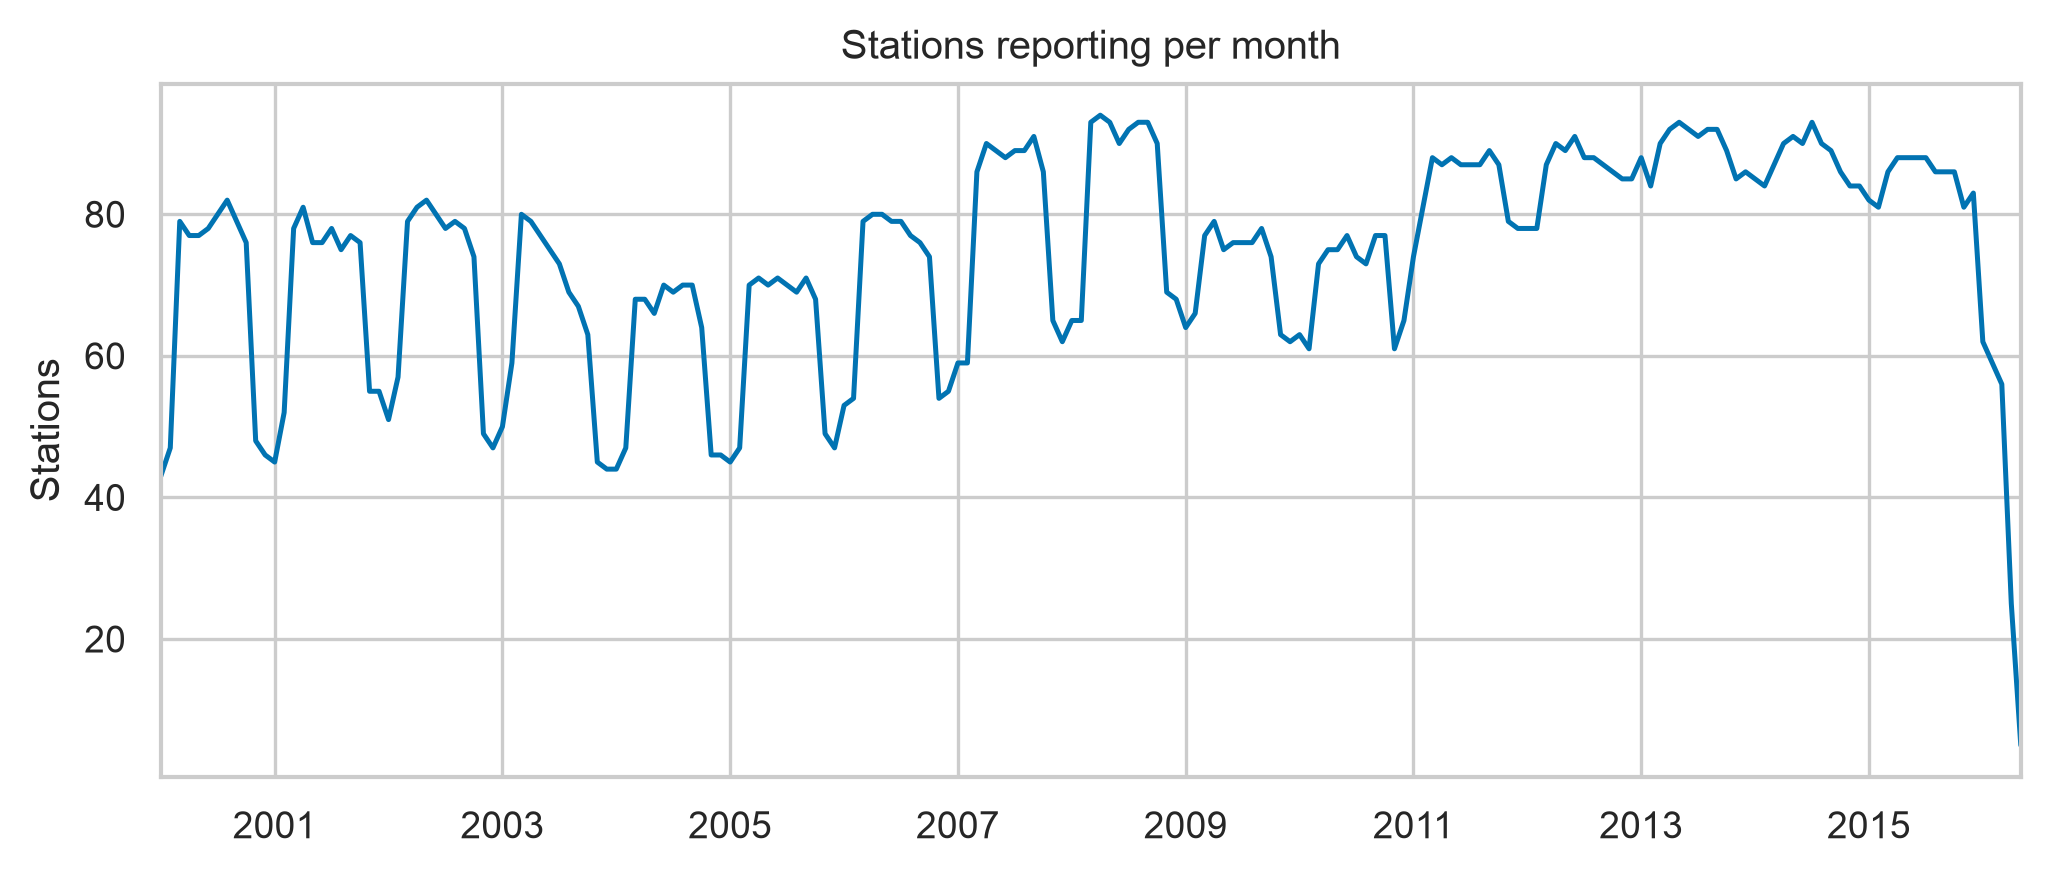
\includegraphics[width=0.9\linewidth]{figures/station_coverage.png}
  \caption{Number of stations reporting O\textsubscript{3} each month.}
  \label{fig:coverage}
\end{figure}

\paragraph{Distributions.} O\textsubscript{3} AQI is centred around 30--40 with a
right tail of high-pollution days reaching about 200. NO\textsubscript{2} is spread
between 0 and 60, while SO\textsubscript{2} and CO are almost always close to zero
(Figure~\ref{fig:distributions}).

\begin{figure}[h]
  \centering
  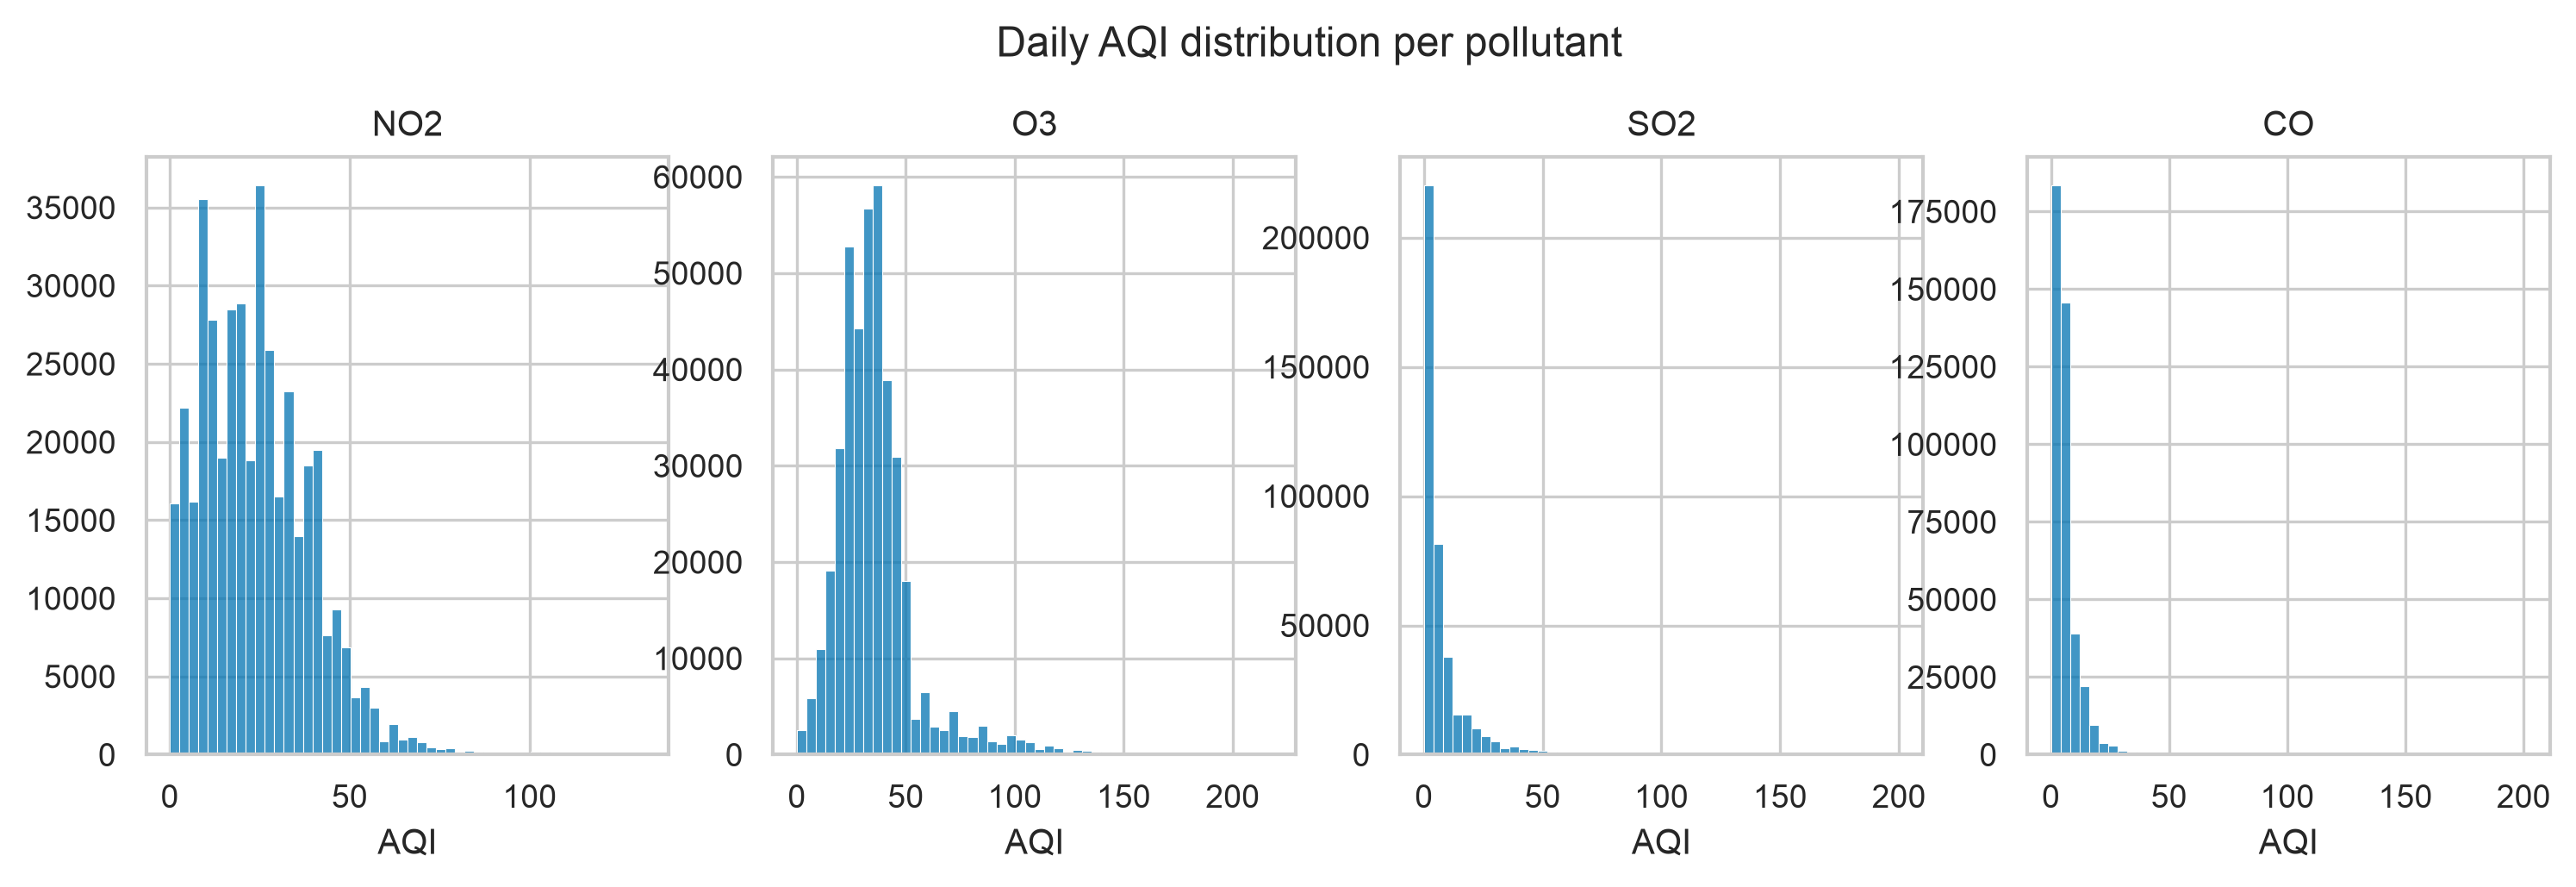
\includegraphics[width=\linewidth]{figures/aqi_distributions.png}
  \caption{Distribution of the daily AQI of each pollutant.}
  \label{fig:distributions}
\end{figure}

\paragraph{Long-term trends.} NO\textsubscript{2}, SO\textsubscript{2} and CO
decrease steadily between 2000 and 2015, whereas O\textsubscript{3} stays flat
at around 35 (Figure~\ref{fig:trends}). Ozone, the pollutant we forecast, has not
improved over the period.

\begin{figure}[h]
  \centering
  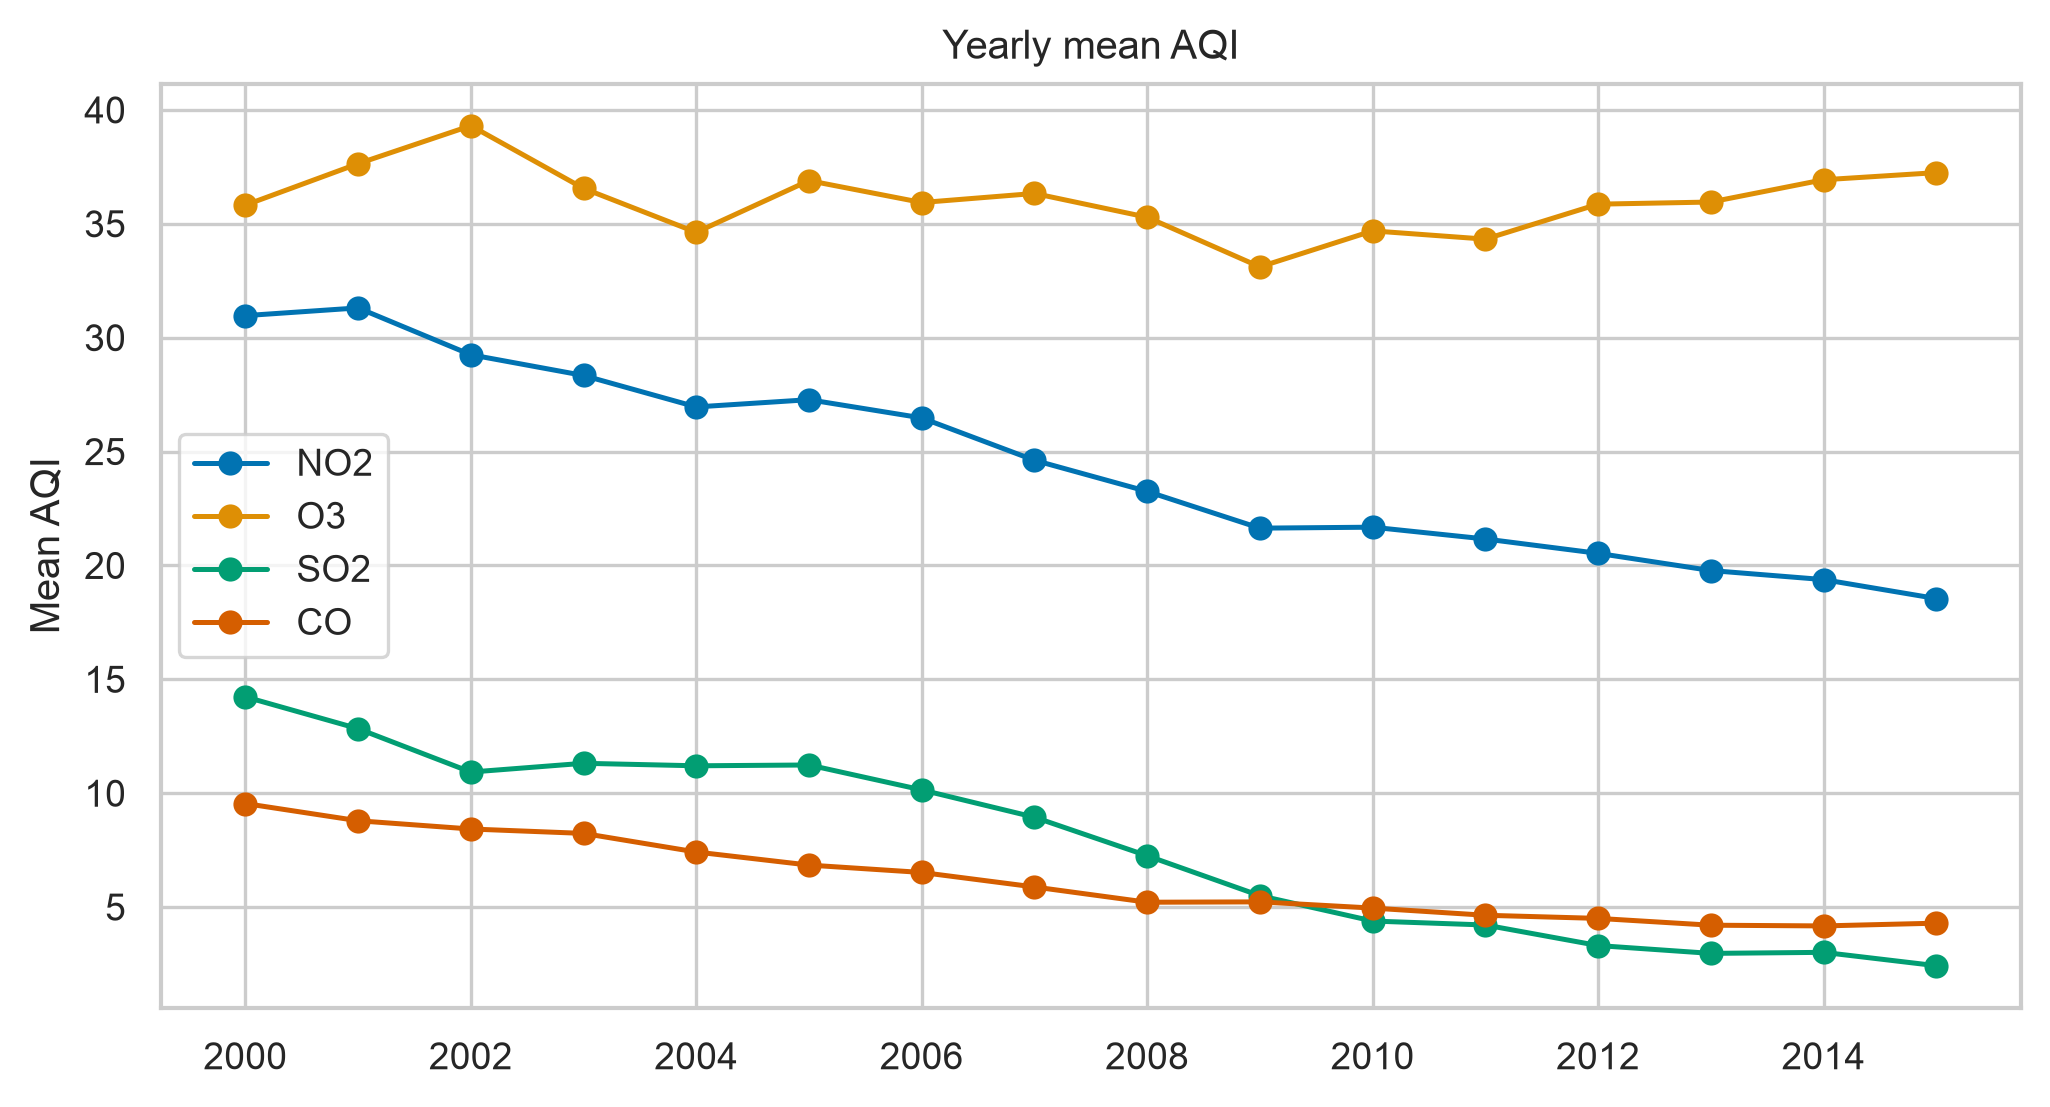
\includegraphics[width=0.8\linewidth]{figures/long_term_trends.png}
  \caption{Yearly mean AQI per pollutant (2016 excluded: only January--May).}
  \label{fig:trends}
\end{figure}

\paragraph{Seasonality.} O\textsubscript{3} peaks in summer (June--August), when
sunlight drives its formation, while NO\textsubscript{2} peaks in winter
(Figure~\ref{fig:seasonality}). NO\textsubscript{2} drops at weekends, consistent
with less traffic, while O\textsubscript{3} rises slightly at weekends. Month and
day of the week are therefore useful features.

\begin{figure}[h]
  \centering
  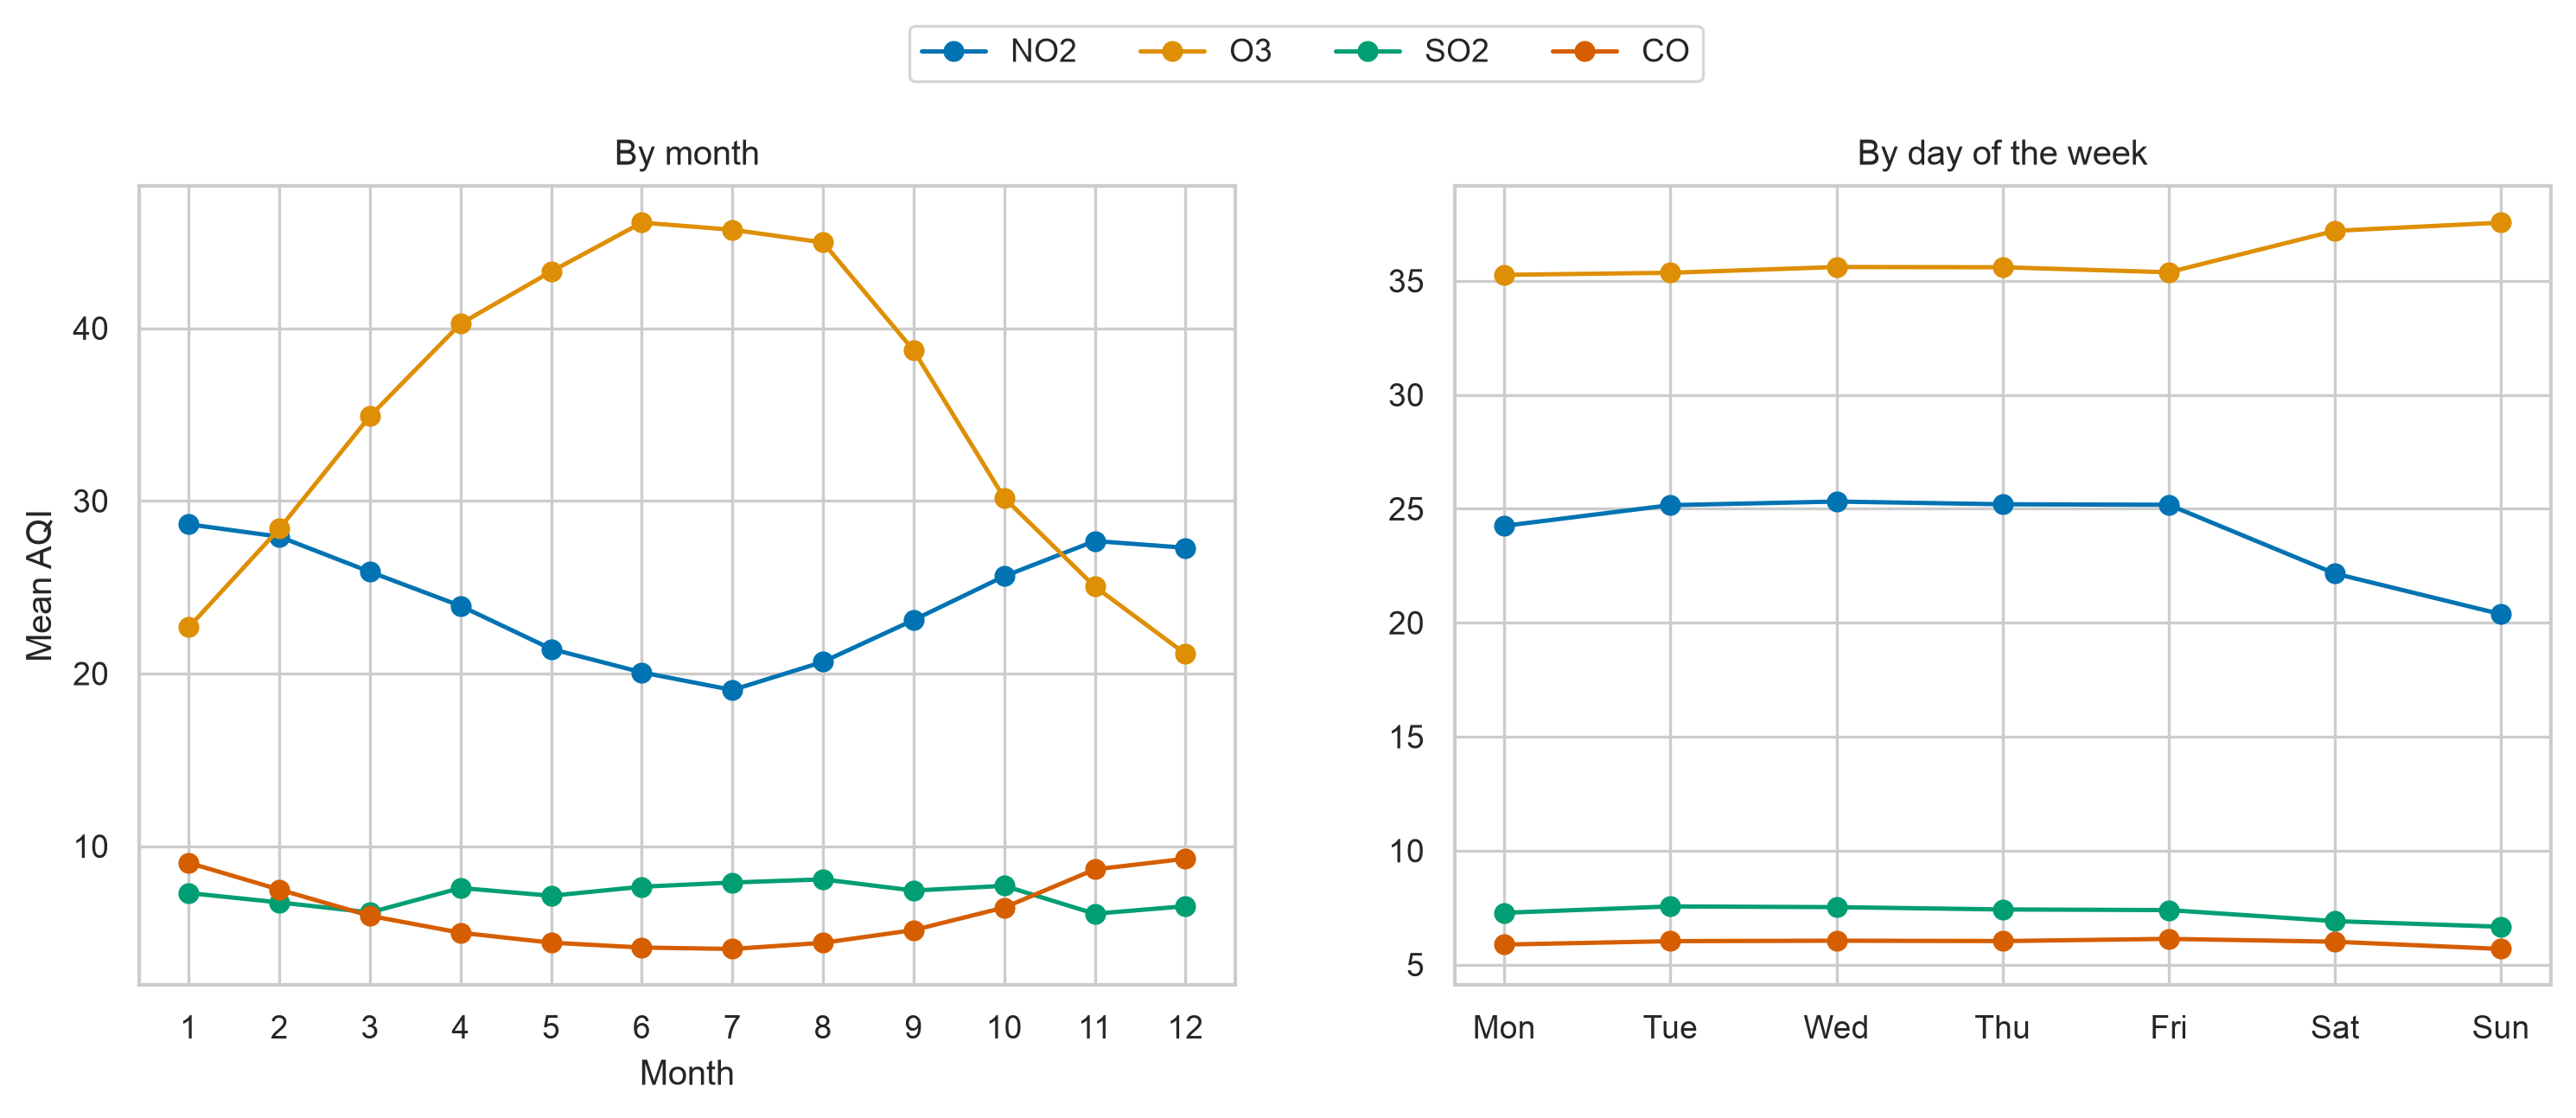
\includegraphics[width=\linewidth]{figures/seasonality.png}
  \caption{Mean AQI by month (left) and by day of the week (right).}
  \label{fig:seasonality}
\end{figure}

\paragraph{Correlations.} O\textsubscript{3} is almost uncorrelated with the other
pollutants, while NO\textsubscript{2} and CO are correlated (0.62), as both come
mainly from traffic (Figure~\ref{fig:correlations}, left). O\textsubscript{3} is
however strongly correlated with its own past: 0.71 with the previous day,
decreasing to about 0.4 after a week (right). This motivates using past values
(lags) as features, and makes ``tomorrow equals today'' a strong baseline.

\begin{figure}[h]
  \centering
  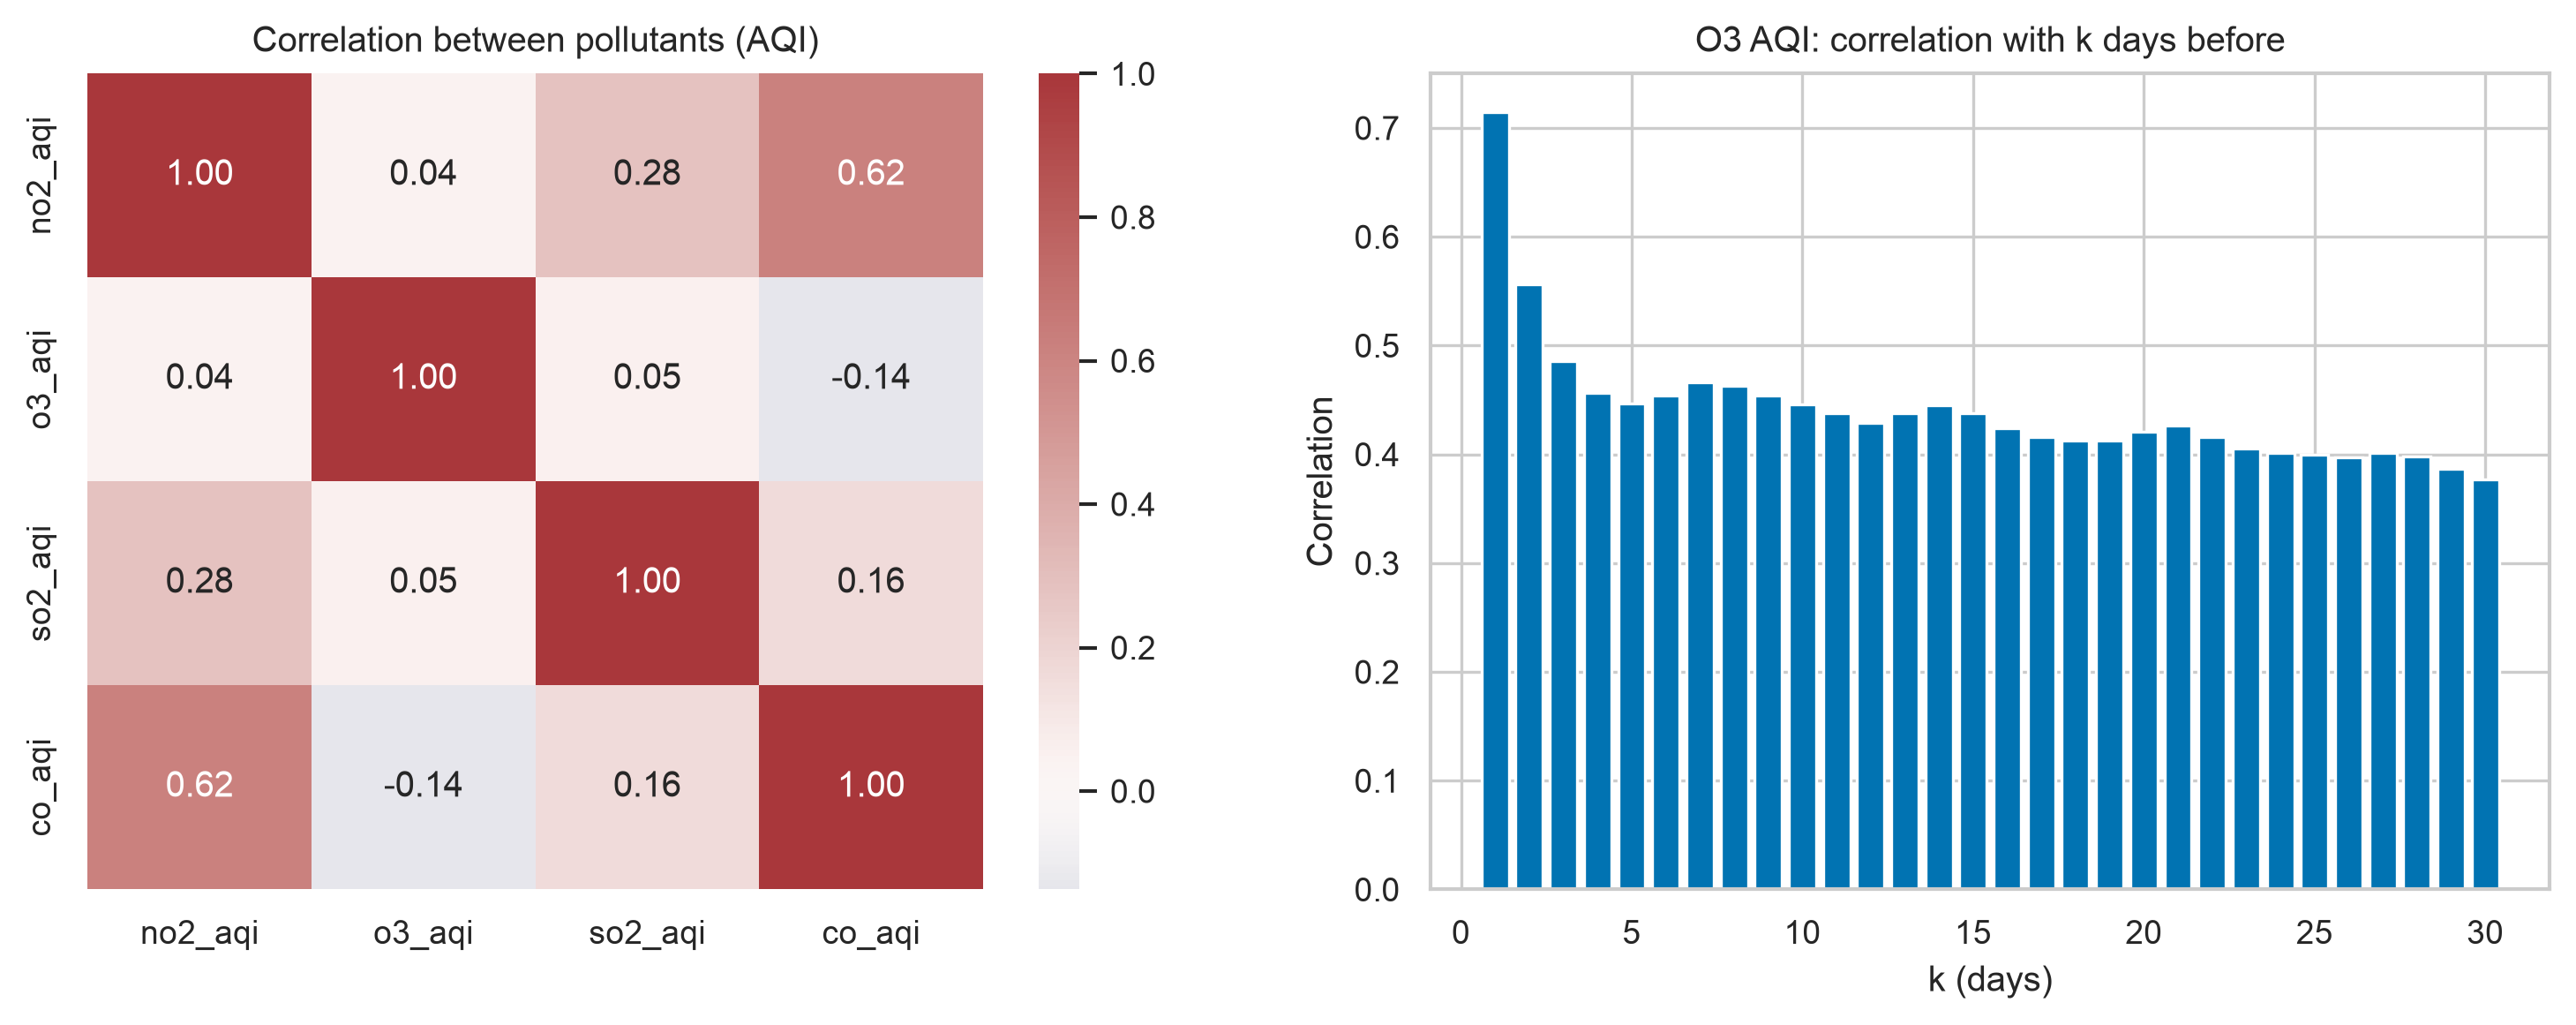
\includegraphics[width=\linewidth]{figures/correlations.png}
  \caption{Left: correlation between pollutants. Right: correlation of
  O\textsubscript{3} AQI with its value $k$ days before, at the same station.}
  \label{fig:correlations}
\end{figure}

\paragraph{Geography.} The mean O\textsubscript{3} AQI varies between states, from
about 45 in Tennessee, North Carolina and Kentucky to below 20 in Alaska
(Figure~\ref{fig:states}). Location therefore carries information.

\begin{figure}[h]
  \centering
  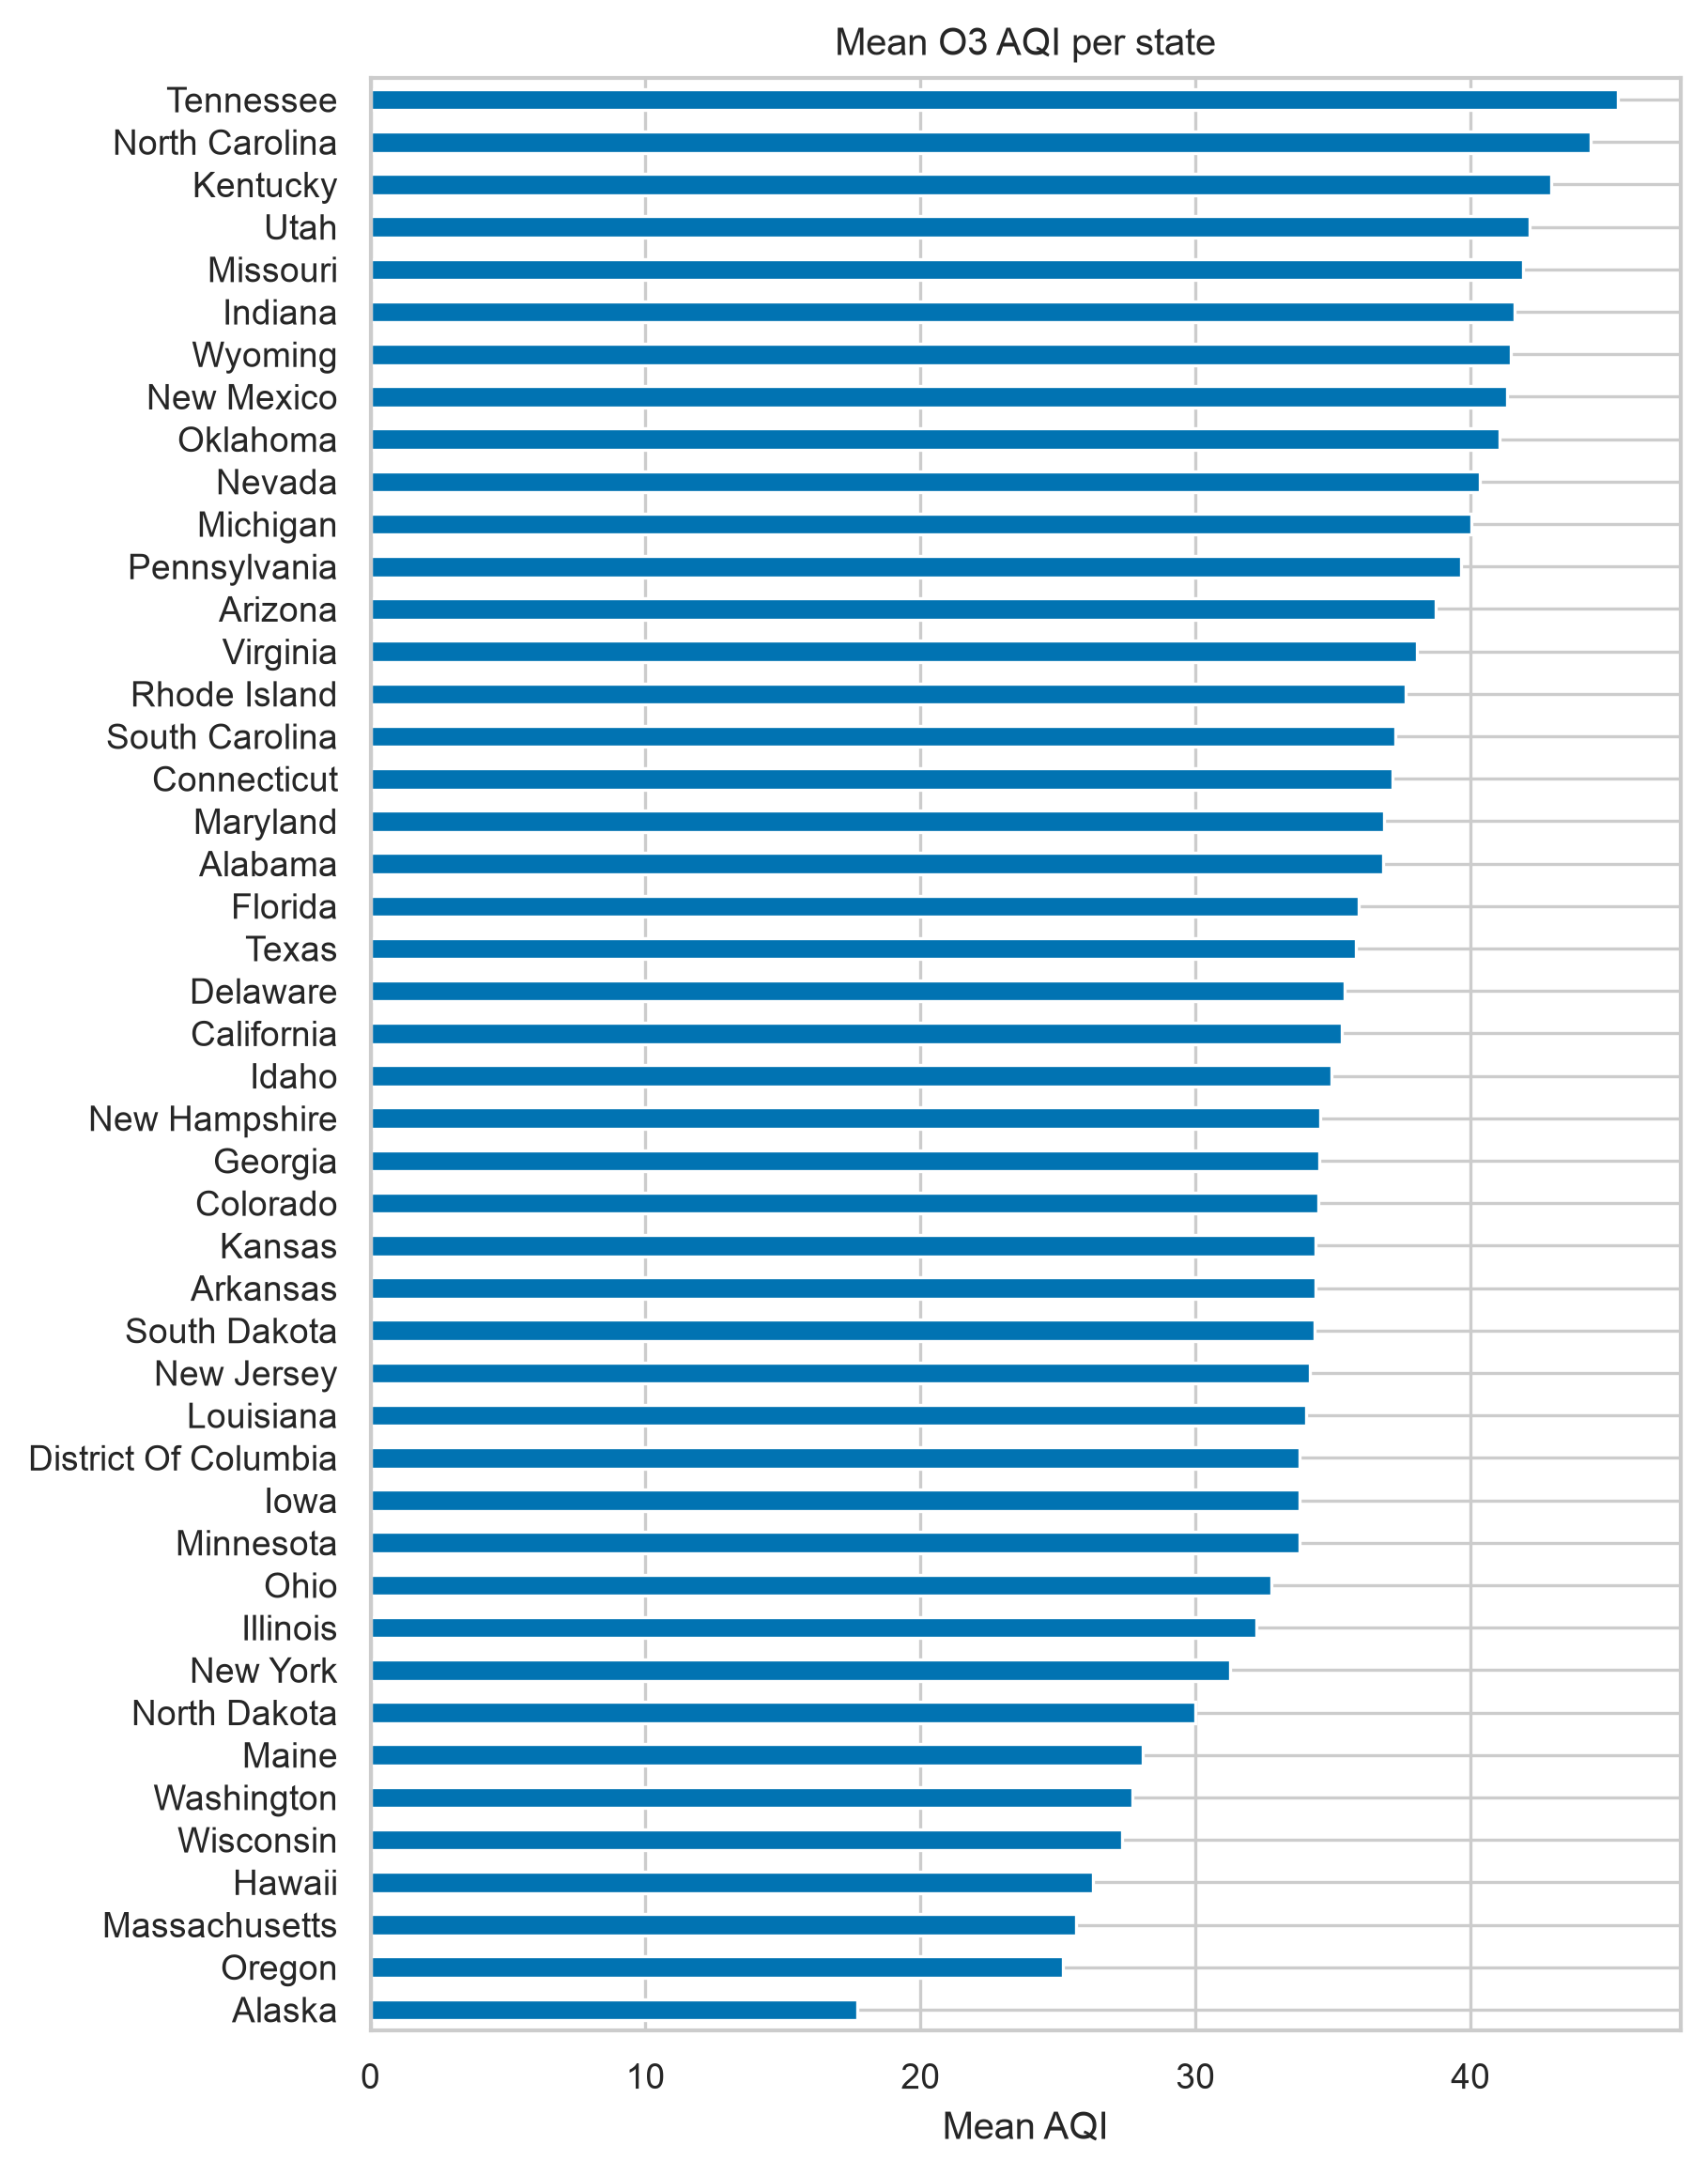
\includegraphics[width=0.6\linewidth]{figures/aqi_by_state.png}
  \caption{Mean O\textsubscript{3} AQI per state.}
  \label{fig:states}
\end{figure}

\section{Theoretical Foundations \& Machine Learning Justification}
% Why each model suits autocorrelated, seasonal, spatially correlated data.
% Validation strategy (time-ordered split, time-series cross-validation) and metrics.
The objective of this project is to develop supervised machine learning models capable of forecasting the next day's ozone air quality index (O3 AQI) at individual monitoring stations across the United States. More precisely, given the historical pollution measurements, temporal information and spatial information available up to day (t), the objective is to estimate the O3 AQI at the same station on day (t+1).\\

\noindent
This can be formulated as a supervised regression problem. Let $s$ denote a monitoring station and $t$ denote a particular calendar day. The target variable can be expressed as:
\begin{equation}
    y(s, t+1)=O3AQI(s, t+1)
\end{equation}
The input vector contains information available at station $s$ on the day before $t$:
\begin{equation}
    X(s,t)=\left[X(s,t)^{\text{temporal }},X(s,t)^{\text{pollutant }}, X(s,t)^{\text{spatial }}\right],
\end{equation}
The forecasting problem is therefore defined as:
\begin{equation}
    \hat{y}(s, t+1)=f(X(s,t))
\end{equation}
where $f$ represents the function learned by the machine learning algorithm and $\hat{y}(s, t+1)$ is the predicted O3 AQI.\\

\noindent
The model is trained using historical observations for which both the input features and the subsequent day's target value are available. During training, the algorithm attempts to identify patterns that explain the relationship between the observed features and the future O3 AQI.\\

\noindent
Unlike a conventional regression problem involving independent observations, this dataset has observations that are organised across both time and geographical locations. Measurements collected at the same station on consecutive dats are not necessarily independent, since atmospheric conditions and pollution concentrations tend to evolve continously. Similarly, stations within the same geographical region may experience related environmental conditions.\\

\noindent
Consequently, the learning problem has spatiotemporal structure. The model must account for temporal persistence, seasonal behaviour and geographical differences, rather than treating each station-day observation as an entirely unrelated sample.\\

\noindent
It is important to distinguish between a conventional spatiotemporal model and a regression model incorporating spatiotemporal features. In this project, spatial and temporal dependencies are represented explicitly through engineered predictors, such as historical pollutant values, calendar variables and the mean O3 AQI of other stations in the same state. The algorithms subsequently learn how these predictors relate to the target variable. This is a feature-based spatiotemporal modelling approach rather than a model that explicitly estimates a continuous spatial process.\\

\subsection{Model selection}
The choice of machine learning algorithms should be motivated by the statistical properties of the underlying data. The exploratory data analysis provides several important observations that influence the selection of appropriate regression methods.\\

\noindent
One of the most relevant findings is the strong autocorrelation of O3 AQI over time. The correlation between the current O3 AQI and its value on the previous day is approximately 0.71, decreasing to approximately 0.4 after one week. This indicates that ozone concentrations exhibit temporal persistence: observations from recent days provide substantial information about the following day's pollution level. This finding justifies including lagged variables and rolling averages in the feature set. However, it also means that the observations cannot be assumed to be statistically independent.\\

\noindent
The algorithms must therefore be evaluated using a methodology that respects chronological order. Randomly distributing observations between training and testing sets could allow information from later periods to influence the training process while earlier observations are used for evaluation, which would not reproduce the intended forecasting scenario.\\

\noindent
The exploratory analysis identifies a clear seasonal pattern in O3 AQI, with higher average values during the summer months. This is consistent with the role of sunlight in photochemical ozone formation. The relationship between atmospheric pollution and calendar variables is therefore not necessarily linear. The use of sine and cosine transformations for the day of the year helps represent the cyclical nature of seasonal behaviour. Nevertheless, the relationship bewtween these seasonal indicators and O3 AQI may involve interactions with historical pollutant concentrations and other temporal variables. This motivates the consideration of nonlinear algorithms capable of identifying complex relationships and interactions without requiring all of them to be specified manually.\\

\noindent
The mean O3 AQI differs considerably between states. This indicates that observations collected at different stations do not necessarily originate from identical statistical distributions. The spatial feature representing the mean O3 AQI of other stations in the same state attempts to capture part of this geographical variation. It provides information about the broader pollution conditions in the station's region, complementing the station's own historical measurements. The inclusion of this feature may help the algorithms identify regional patterns that cannot be explained exclusively by individual station histories.\\

\noindent
The correlation analysis between pollutants indicates that the predictive contribution of each pollution should not be assumed to be identical. Although O3 formation is influenced by atmospheric chemistry involving precursor pollutants and environmental conditions, a simple linear association between daily AQI measurements does not necessarily capture these mechanisms. Consequently, models should be capable of determining whether pollutant measurements contribute to prediction through nonlinear relationships or interactions with other features.\\

\noindent
The dataset also contains a substantial amount of missing station-day information. This creates an important modelling constraint. Missing observations should not automatically be interpreted as zero pollution. The algorithms must therefore be trained using an appropriate missing-data strategy. Depending on the implementation, this may involve restricting training to observations with complete required features, imputing selected predictors using information available at the prediction time, or using an algorithm with native missing-value handling.\\

\noindent
The missing-data treatment must be fitted using training data only where applicable, so that information from the test period does not influence the training process.\\

\noindent
Overall, these characteristics suggest that a single simple linear relationship may not adequately describe the forecasting problem. It is therefore methodologically appropriate to compare a simple statistical baseline, a regularised linear regression model and non-linear ensemble-based methods.

\subsection{Baseline Model: Persistence Forecast}
The natural baseline for this project is the persistence forecast. The assumption is that the next day's O3 AQI will be equal to the current day's O3 AQI:
\begin{equation}
    \hat{y}(s, t+1)=y(s,t)
\end{equation}
\noindent
This model does not attempt to learn a complex relationship between several explanatory variables. Instead, it assumes that the most recent observation is the best available estimate of the next observation. The methodological justification for this baseline comes directly from the exploratory data analysis, which indicates substantial temporal dependence. Therefore, predicting tomorrow's value using today's value is a meaningful reference point rather than an arbitrary benchmark.\\

\noindent
The persistence model is particularly useful because it allows the performance of more advanced algorithms to be interpreted in context. A model achieving a relatively low prediction error is not necessarily useful if it cannot improve upon the simple assumption that pollution levels remain approximately unchanged from one day to the next.\\

\noindent
However, the persistence model has important limitations. It cannot explcitly account for seasonal transitions, geographical differences, interactions between pollutants or nonlinear changes in atmospheric conditions. It also cannot generate a prediction when the required previous-day O3 AQI is unavailable unless an additional missing-data strategy is introduced. For these reasons, the persistence forecast is not intended to be the final predictive model. Its purpose is to establish a minimum performance benchmark that more sophisticated methods should outperform.\\

\subsection{Regularised linear regression}
Linear regression is one of the fundamental approaches to supervised regression. It assumes that the expected value of a continuous target variable can be represented as a linear combination of the input features.\\

\noindent
For an observation $i$, the model can be expressed as
\begin{equation}
    y_i=\beta_0+\sum_{j=1}^p\beta_jx_{ij}+\varepsilon_i
\end{equation}
where $y_i$ represents the observed O3 AQI, $x_{ij}$ represents the value of feature $j$ for observation $i$, $\beta_0$ is the intercept, $\beta_j$ represents the coefficient associated with feature $j$, $p$ is the total number of input features and $\varepsilon_i$ represents the unexplained component of the target variable.\\

\noindent
The model estimates the coefficients by minimising the sum of squared residuals between observed and predicted values:
\begin{equation}
    \min_\beta\sum_{i=1}^n(y_i-\hat{y}_i)^2
\end{equation}
\noindent
The resulting model provides a relatively simple representation of the relationship between the explanatory variables and the target. Its principal advantage is interpretability. Each coefficient represents the estimated change in the prediction associated with a one-unit change in the corresponding feature, conditional on the remaining features being held constant. This interpretation describes an association learned by the model, not necessarily a causal relationship.\\

\noindent
Although the exploratory analysis suggests nonlinear relationships, linear regressions remains an important methodological reference. First, the dataset contains several features that may exhibit approximately linear predictive relationships with the tarder over certain ranges. In particular, historical O3 AQI measuremens may provide a strong linear signal because of the observed temporal autocorrelation. Second, the model provides an interpretable way of examining the contribution of temporal, spatial and pollutant-related features. Third, linear regression offers a useful comparison against more complex algorithms. If a nonlinear model achieves substantially better performance, this provides evidence that the additional flexibility is useful for capturing relationships that a linear model cannot adequately represent. If the performance improvement is small, a simpler model may be preferable because it is easier to interpret and computationally less demanding.\\

\noindent
A potential problem with ordinary leat squares regression is multicollinearity, which occurs when two or more explanatory variables are strongly correlated. In this project, several features are likely to contain overlapping information. When predictors are highly correlated, ordinary least squares coefficients can become unstable. Small changes in the training observations may produce substantial changes in the estimated coefficients, making individual coefficient interpretations less reliable. Regularisation provides a way to address this problem. A suitable extension is Ridge Regression, which adds a penalty to the ordinary least squares objective:
\begin{equation}
    \min_\beta\left[\sum_{i=1}^n(y_i-\hat{y}_i)^2+\lambda\sum_{j=1}^p\beta_j^2\right]
\end{equation}
\noindent
where $\lambda$ controls the strength of the regularisation. The penalty discourages excessively large coefficients by shrinking their magnitudes towards zero. Unlike Lasso regression, Ridge Regression generally retains all predictors rather than forcing some coefficients to become exactly zero. This is particularly appropriate when multiple features contain overlapping predictive information. For example, different historical lags may all contribute to the prediction, even if their individual contributions cannot be estimated reliably without regularisation. The regularisation parameter should be selected using validation data, preferably though chronological cross-validation. Continuous predictors should also be standardised before applying Ridge regression, since the penalty is sensitive to the scale of the coefficients. Scaling parameters must be estimated from the training data only.\\

\noindent
Linear regression relies on several assumptions that should be considered when interpreting its predictions. The first one is linearity, as the expected target value is assumed to be a linear function of the predictors. The second one is independence of errors, as residuals are assumed to be independent for conventional statistical inference. The residual variance is assumed to remain approximately constant across observations, explanatory variables should not be correlated with the unexplained error ccomponent for standard coefficient interpretations, and lastly predictors should not exhibit problematic levels of linear dependece. In particular, temporal dependence may lead to correlated residuals, and the relationships between O3 AQI and seasonal variables may be nonlinear.\\

\noindent
It is important to note that violations of these assumptions do not automatically make linear regression unusuable for prediction. However, they can affect its predictive performance and the validity of conventional statistical inference. Therefore, regularised linear regression is primarily included as an interpretable benchmark and a way of evaluating whether a relatively simple functional relationship can explain a meaningful proportion of the observed variation.

\subsubsection{Random forest regression}
Random forest is an ensemble learning algorithm based on decision trees. An ensemble method combines the predictions of multiple individual models to produce a final prediction that is generally more robust than relying on a single model. A decision tree divides the feature space into a collection of regions using a sequence of decision rules. The final prediction is obtained from the observations belonging to the terminal region, usually through the average target value of the training observations in that region.\\

\noindent
In regression, the objective of the tree-building procedure is generally to identify splits that reduce the variation of the target variable within the resulting groups. A single decision tree can capture nonlinear relationships and interactions between variables. However, individual trees are often sensitive to changes in the training data, which can result in high prediction variance. Random forest addresses this limitation by constructing a large collection of decision trees and combining their predictions.\\

\noindent
The algorithm introduces randomness through two main mechanisms. First, eachh tree is trained using a bootstrap sample of the original training observations. This means that observations are sampled with replacement, producing different raining subsets for different trees. Second, the algorithm considers at each split a randomly selected subset of the available features rather than evaluating every feature. These mechanisms reduce the correlation between individual trees and help prevent the ensemble from depending excessively on a small number of predicors.\\

\noindent
For regression, the final prediction is calculated as the average prediction of all trees
\begin{equation}
    \hat{y}(x)=\frac{1}{B}\sum_{b=1}^BT_b(x)
\end{equation}
where $B$ is the number of trees in the forest and $T_b(x)$ is the prediction generated by tree $b$ for input vector $x$. Averaging across multiple trees generally reduces the variance associated with individual decision trees, improving the stability of the predictions.\\

\noindent
Random forest is methodologically attractive for this project because the relationship between O3 AQI and its explanatory variables is unlikely to be entirely linear. The first relevant characteristic is the nonlinear nature of atmospheric pollution dynamics. A decision tree can represent such relationships through treshold-based splits without requiring the modeller to specify a particular mathematical functional form in advance. The second advantage is the ability to capture interactions between features, as random forest can identify these interations through successive splits in the decision trees.\\

\noindent
Another important advantage is that random forest does not require predictors to be normally distributed or linearly related to the target. This is useful because the exploratory analysis identifies a right-skewed O3 AQI distribution, with most observations concentrated around 30-40 and a smaller number of high-pollution days reaching approximately 200.\\

\noindent
Furthermore, the method can workd with features measured on different numerical scales wihout requiring standardisation as a mathematical prerequisite. This is particularly useful when combining AQI measurements, calendar variables and spatial averages. Random forest can also provide feature-importance estimates, allowing an initial examination of which predictors contribute most to the model's predictive performance. However, feature importance should be interpreted carefully. Correlated predictors can distribute or distort importance scores, and a high importance score does not imply a causal relationship.\\

\noindent
Unlike a linear regression, random forest does not assue a globally linear relationship between the predictors and the target.  Nevertheless, it has its own limitations.\\

\noindent
First, decision trees divide the feature space into regions and produce piecewise-constant predictions. Consequently, they may not represent smooth changes in atmospheric conditions as naturally as some other regression methods. Second, random forest does not explicitly model temporal order or spatial dependence. The algorithm only recognises theses relationships through the engineered features supplied to it. This means that the quality of the temporal lags, rolling averages and spatial aggregation features remains essential. Third, predictions outside the range target calues observed during training are generally difficult for standard regression forests to produce. This may be relevant when forecasting unusually high pollution episodes that are poorly represented in the training data. Finally, random forest ccan require considerable computational resources when trained using many trees and a large dataset. Despite these limitations, it provides a useful compromise between predictive flexibility, robustness and the ability to model complex interactions.

\subsubsection{Gradient boosting regression}
Gradient boosting is another ensemble learning method based on decision trees. Unlike random forest, which builds multiple trees independently and averages their predictions, gradient boosting constructs trees sequentially. Each new tree is trained to improve the predictions produced by the existing ensemble. The central idea is to build an additive model in which successive learners correct part of the remaining prediction error.\\

\noindent
For a regression problem, the model can be expressed as
\begin{equation}
    F_M(x)=F_0(x)+\sum_{m=1}^M\nu h_m(x)
\end{equation}
where $F_0(x)$ is the initial prediction, $h_m(x)$ is the regression tree added at iteration $m$, $M$ is the total number of boosting iterations and $\nu$ is the learning rate, controlling the contribution of each new tree.\\

\noindent
For squared-error regression, the initial prediction is commonly the mean target value in the training data. The algorithm then calculates the residuals between the observed values and the current predictions
\begin{equation}
    r_i=y_i-F_{m-1}(x_i)
\end{equation}
The next tree is trained to approximate these residuals, allowing the ensemble to improve its predictions. More generally, gradient boosting can be understood as a numerical optimization procedure in function space. Instead of directly optimizing as a fixed set of regression coefficients, it progressively constructs a funcion that minimises a chosen loss function. \\

\noindent
For squared-error regression, the objective is:
\begin{equation}
    L(y, F(x))=\frac{1}{2}(y-F(x))^2
\end{equation}
\noindent
The negative gradient of this loss with respect to the current prediction is proportional to the residual. Therefore, fitting a new tree to the residuals corresponds to taking a step towrds reducing the prediction error. The learning rate controls the size of these steps. A smaller learning rate generally requires more boosting iterations but can produce a more gradual optimization process.\\

\noindent
Gradient boosting is particularly relevant because the dataset contains multiple sources of potentially nonlinear predictive information. The relationship betweem recent O3 AQI measurements and the next day's target may vary depending on seasonal conditions, geographical location and other pollutant measurements. Gradient boosting can approximate these complex relationships by combining successive decision trees.\\

\noindent
Its sequential learning strategy is especially useful when a relatively simple model leaves systematic patterns in the residuals. For example, an initial tree may capture the general relationship between the previous day's ozone concentration and the following day's value. Subsequent trees can then improve predictions for observations with particular seasonal or spatial characteristics that the first tree did not adequately represent.\\

\noindent
Another advantage is its flexibility with respect to the loss function. Squared-error loss is a natural starting point for continuous AQI prediction because it penalises large deviations more heavily than small ones. However, the right-skewed distribution of O3 AQI suggests that a small number of igh-pollution observations may contribute substantially to the overall squared error.\\

\noindent
Gradient boosting has several important hyperparameters that control the balance between model complexity and generalisation.

\section{Model Implementation \& Performance Evaluation}
% Baselines vs. advanced models, hyperparameter tuning, validation and test results.

\section{Challenges, Enablers \& Lessons Learned}

\section{Individual Contribution Breakdown}
\begin{tabular}{@{}lp{10cm}@{}}
\toprule
Member & Role, responsibilities and tasks \\
\midrule
TODO & TODO \\
TODO & TODO \\
TODO & TODO \\
\bottomrule
\end{tabular}

\appendix
\section{Declaration of Generative AI Tool Usage}
% Mandatory. Summarise docs/ai_usage_log.md: tools, key prompts, scope of help,
% and at least one example of incorrect/suboptimal AI output and how it was fixed.

\end{document}